\section{Hypothesis and Implement} %6.2
Referencing Figure~\ref{4_1_1_without2} in Subsection~\ref{subsection4.1.1}, we find one of the lowest point, as shown in the Figure~\ref{6_2_g9}, as our start point of Emergency Control.  

\begin{figure}[htbp]
\centering
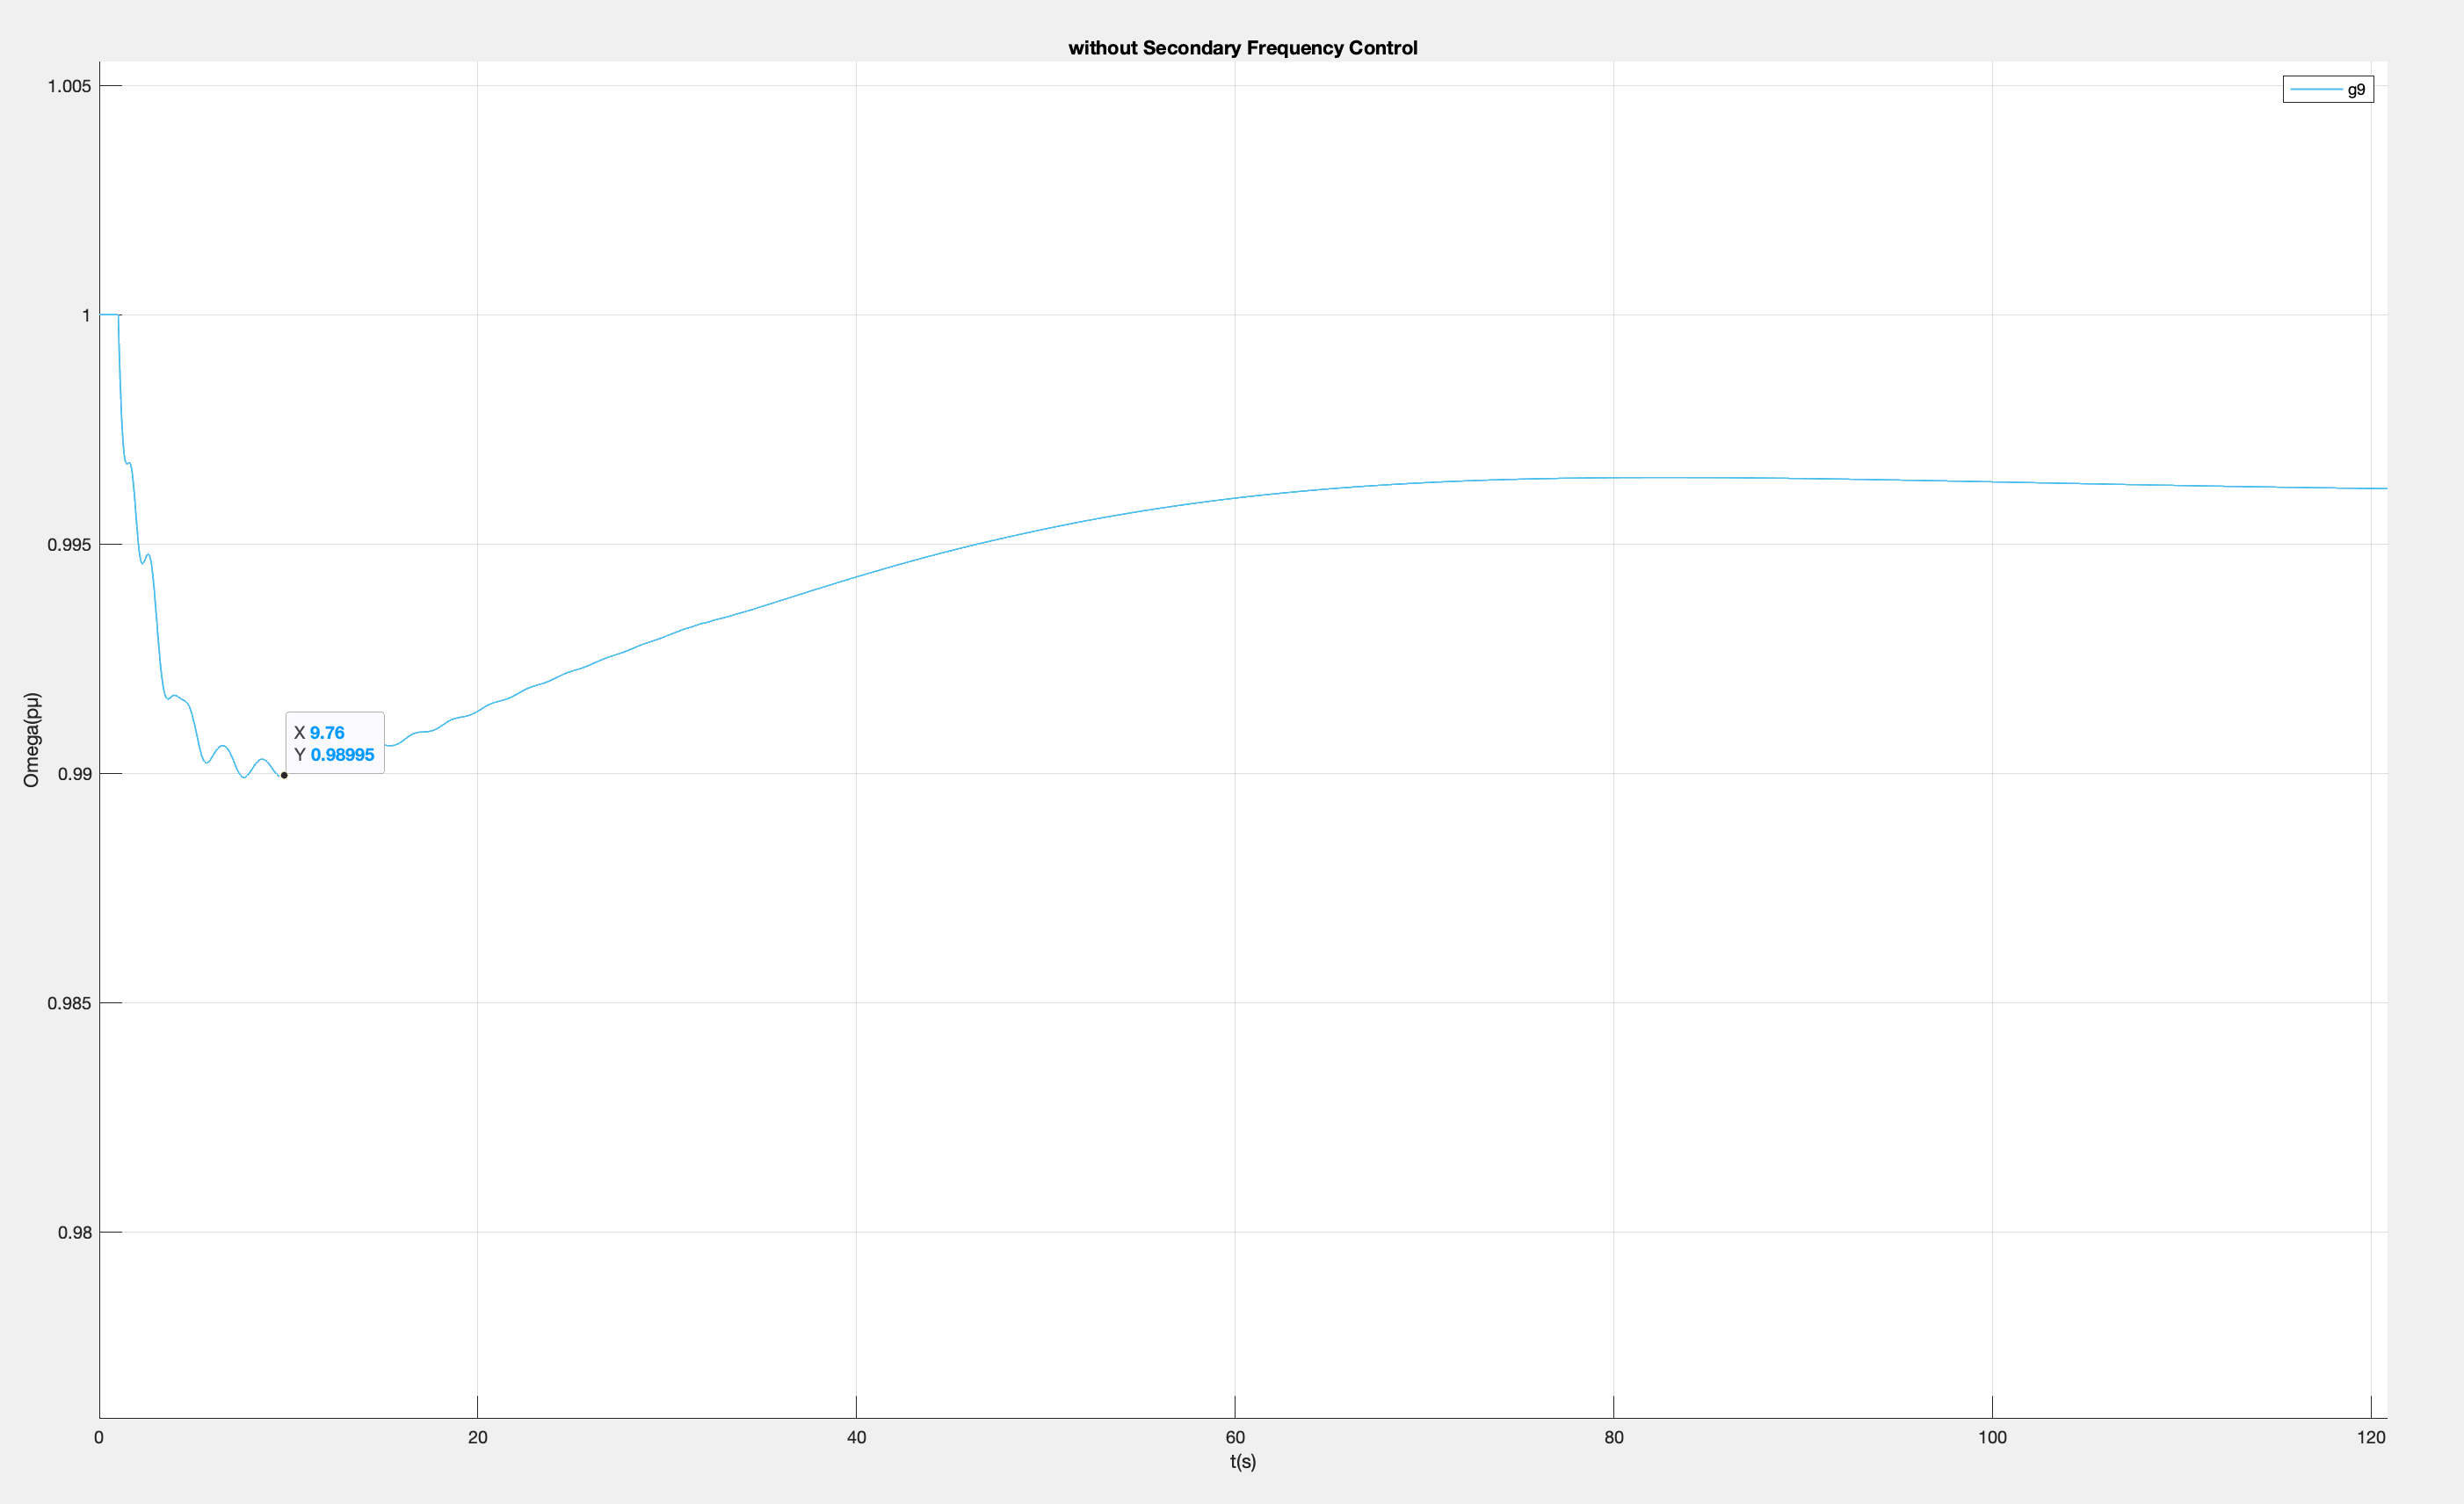
\includegraphics[width = .819\textwidth]{figure/6_2_g9.png}
\caption{Start time of Emergency Control.}
\label{6_2_g9}
\end{figure}

We start the Emergency Control from the 9.76th second and use one of the acceptable tuning results, i.e. kp is 30.1 and ki is 0.1, in Chapter~\ref{Chapter4}. The aim of such hypothesises is to test the impact of time delay under the condition of Emergency Control. The simulation lasts for 360 seconds. 